\subsection{Edge Computing}

Das Ziel hinter Edge Computing ist es zum einen, Rechen oder Speicher Ressourcen näher an die Clients zu bringen. Edge Computing Server dienen dabei als Schnittstelle zwischen IoT Geräten und Datenzentren die sich in der Cloud befinden können \cite{luntovskyyHighlyDistributedSystemsIoT2022}.\\
Das Konzept wurde im modernen Kontext erstmals 2012 in einem Paper von dem Unternehmen Cisco vorgestellt \cite{bonomiFogComputingIts}. Dabei wurde es als Erweiterung der Cloud zur Unterstützung von Internet of Things (IoT) Anwendungen definiert. Anzumerken sei, dass im Paper der Begriff 'Fog' für 'Edge' genutzt wird. Beide werden in der Literatur oftmals als Synonym genutzt. In dieser Arbeit, wird der Begriff 'Edge' eingesetzt.\\
Wie also beschrieben, ist das Edge Computing eine besondere Art der Bereitstellung von Ressourcen für Clients. Aus diesem Grund, kann man mehrere Eigenschaften ausmachen die für das Edge computing von Bedeutung sind\cite{bonomiFogComputingIts}:

\begin{enumerate}
  \item Standorts Bewusstsein und geringe Latenz: Edge Knoten werden vornehmlich in der Näher von Clients plaziert. Dadurch können diese entlastet werden ohne dass es zu großen Latenz Problemen kommt.
    \item Geografische Verteilung: Um die nähe der Clients zu gewährleisten, werden die Edge Knoten an verschiedenen Orten angebracht. Dies muss beim Deployment der Knoten beachtet werden.
      \item Beweglichkeit: Im gegensatz zu stationäre Server, sind Edge Instanzen in Ihrem Ort beweglich. Dies ist nötig um Clients an unterschiedlichen Orten zu unterstützen und flexibel zu bleiben. Dafür wird ein System gebraucht welches den jeweiligen Edge Host von seinem Ort entkoppelt und Änderungen am Standort wahrnimmt und unterstützt.
        \item Echtzeit Kommunikation: Edge Knoten müssen in Echtzeit mit Endanwendungen kommunizieren können. Eine Verarbeitung in Form von zum Beispiel eine Warteschlange ist hier nicht möglich, da Clients auf die Antwort des Edge Servers womöglich angewiesen sind.
\end{enumerate}

Edge Computing unterscheidet sich dabei in verschiedenen Aspekten vom regulären Cloud Computing. Verbindungen haben in diesem Kontext oftmals eine viel größere Lebensspanne. Das heißt, dass die Verbindungen nicht wie bei regulären Internetdiensten nach einer kurzen Zeit wieder geschlossen werden. Ebenfalls, gibt es im Bereich des Edge Computings sehr viele heterogene Clients. Im Kontext der Robotik, könnte man zum Beispiel Verbindungen von einem mobilen Roboter und einem stationären Greifarm unterscheiden. Besonders eindrucksvoll ist dies im IoT Bereich, in dem man sehr viele verschiedene Verbindungen verarbeiten muss.\\
Diese Eigenschaften haben verschiedene Vorteile gegenüber dem regulären Cloud Computing. Einerseits, kann eine kürzere Distanz zum Server die Latenz der Verbindungen verbessern. Andererseits, kann es zu einer direkten Datenannahme und Pre-Prozessierung der Daten direkt am Standort kommen. Dies ist hilfreich, wenn die Datenverarbeitung für die Funktionalität des Roboters von Relevanz ist \cite{luntovskyyHighlyDistributedSystemsIoT2022}.

\begin{figure}
  \centering
  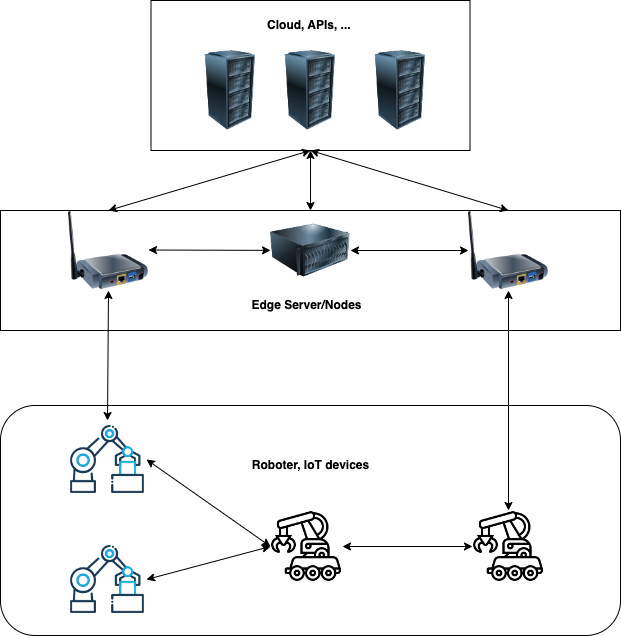
\includegraphics[width=0.5\textwidth]{./figures/edge-computing.png}
  \caption{Vereinfachte Edge Computing Architektur}
  \label{fig:edge-computing}
\end{figure}

Trotz der Allgegenwärtigkeit von Cloud Computing Services in unserem Alltag\cite{GartnerForecastsWorldwide2022}, gibt es im Edge Computing Bereich noch einige Herausforderungen. Eine davon ist die Konnektivität zwischen den Edge Knoten und den jeweiligen Geräten wie beispielsweise den Robotern. Das Wunschszenario wären hier hohe Datenraten mit möglichst niedrigen Verbindungsverzögerungen \cite{groshevEdgeRoboticsAre2022}. Dies ist aber oftmals durch äußere Einflüsse nicht reibungslos möglich. Beispielsweise spielt die Standort Wahrnehmung hier eine Rolle. Ein Roboter, der sich näher am Edge Knoten befindet kann auch von einer besseren Konnektivität profitieren.

Ziel ist es also die Zusammenarbeit zwischen Heterogene Ressourcen wie beispielsweise Roboter und Edge Knoten zu verbessern. Dafür müssen verschiedene Variablen berücksichtigt werden. Unter anderem die Konnektivität, die geographische Verteilung der Knoten oder der spezielle Use Case der umgesetzt werden soll.\\
In \ref{fig:edge-computing} ist eine vereinfachte Edge Architektur dargestellt. Hier hat man in der untersten Schicht mehrere Roboter die Dienste von einer Edge Instanz nutzen. Die Edge Instanzen können sich dabei direkt bei den Robotern befinden (Bspw. in einer Fabrik) oder nur geographisch an einem nähern Ort als Cloud Server. Durch die nähere Distanz ist aus performance Sicht eine Auslagerung überhaupt möglich. In der obersten Schicht, sind die für Roboter Betriebs irrelevante Services angesiedelt. Diese können zum Beispiel Cloud Schnittstellen sein, die Berechnungen anhand der gesammelten Daten an der Edge ausführen.
